\documentclass[11pt, a4paper]{article}
\usepackage[utf8]{inputenc}
\usepackage[left=2cm, right=2cm, top=2.5cm, bottom=2.0cm]{geometry}
\usepackage{amsmath, amssymb, amsthm}
\usepackage[english]{babel}
\usepackage{graphicx}
\usepackage[font={small,it}]{caption}
\graphicspath{ {figures/} }
\usepackage{url}
\usepackage{appendix}
\usepackage{float}
\usepackage{multirow}
\usepackage[bottom]{footmisc}
\usepackage{wrapfig}
\usepackage{subcaption}
\usepackage{titling}
\setlength{\droptitle}{-10em}  

\usepackage{titling}


\title{ \huge Artificial neural networks \\ 
  { \large Assignment 2: Bayesian learning in neural networks }}
\author{
        Lood, Cédric \\
        \small Master of Bioinformatics
}

\begin{document}
\maketitle
%\tableofcontents

\section{Context}
Bayesian statistics offer a robust framework in which it is possible
to build and assess models, and perform inference. 

In this exercise, we explore bayesian learning applied to neural
networks. Using the Bayes rule in the context of learning has several
desirable properties related to the fact that one is not using point
estimates in the search space of solutions (for example the weight
space) but tries to obtain a distribution over the weight
space. Hence, quantification of certainty of predictions is possible
without the use of validation set or resampling.

\section{Decision boundary of classifier}

In this section, I investigated whether a simple bayesian approach
(MAP) could classify correctly data generated by a perceptron (hence
linearly separable). In terms of architecture, the perceptron created
consisted of 1 neuron with 2 inputs taking values in $[-1; 1]$,
without bias term. The output of the perceptron is in $\{-1, 1\}$

Figure \ref{fig:perceptron_bayes} displays the classifiers on top of
the dataset (top left-hand side figure). You can see that the
classifier generated using the Bayes rule sits close to the perceptron
used to generate the dataset. There seemed to be exceptions to that,
and in a few cases the classifier was really off.

To note, starting with a gaussian prior, the convergence of the
posterior through the iterative updates always entailed that one of
the weight (w1 or w2) was set to 1, while the other varied. I did not
see exception to that when running the script multiple times. The MAP
weights of the bayesian classifier were often close to that of the
perceptron, but given that there is an infinite amount of possible
classifiers for this dataset, multiple combinations are possible. It
also happened that the bayesian approach did not reach a 100\% correct
classification (see top left graph).

\begin{figure}[H]
    \centering
    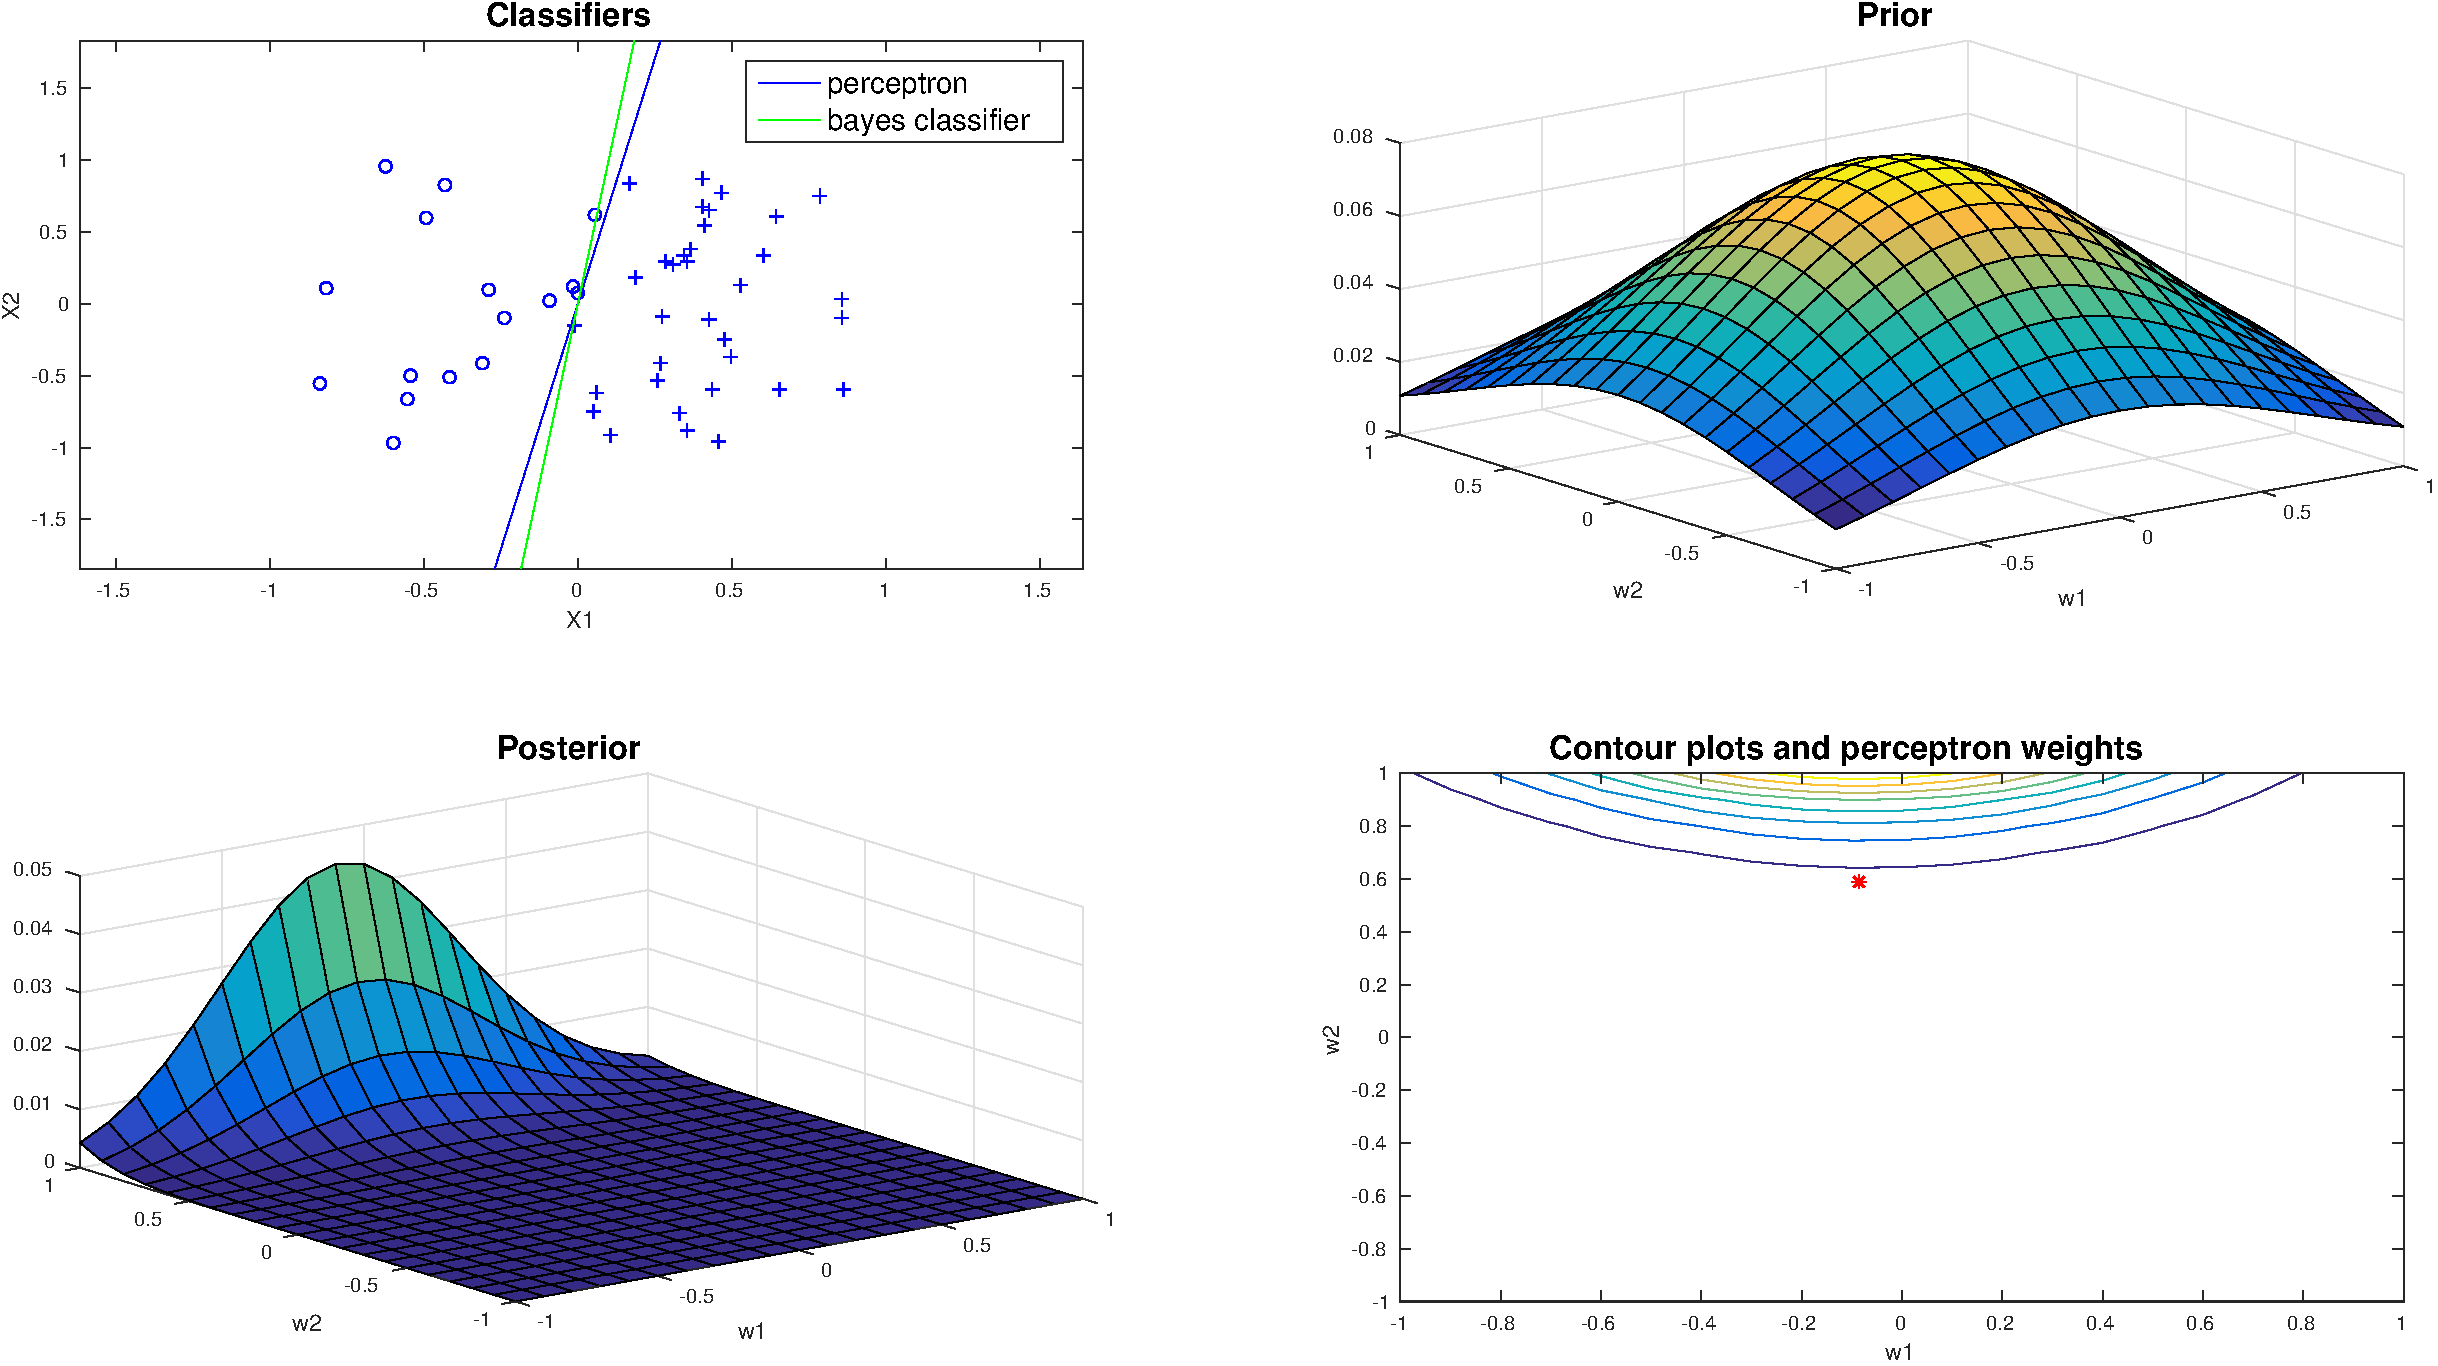
\includegraphics[scale=.40]{perceptron_bayes.pdf}
    \caption{Comparison of perceptron and bayes classifier for dataset
      generated by perceptron}
    \label{fig:perceptron_bayes}
\end{figure}

\section{Function approximation}

The underlying function considered in this section is $f(x)=sin(x)$,
with some gaussian noise added for the training dataset. On figure
\ref{fig:trainbr}, you can see the results of the function
approximation using \emph{trainlm} and \emph{trainbr} using different
amounts of neurons (but a fixed amount of epochs). 

The effects of bayesian as regularization can be seen, as the
overfitting seems lower compared to the \emph{trainlm} approach. 

\begin{figure}[H]
  \centering
  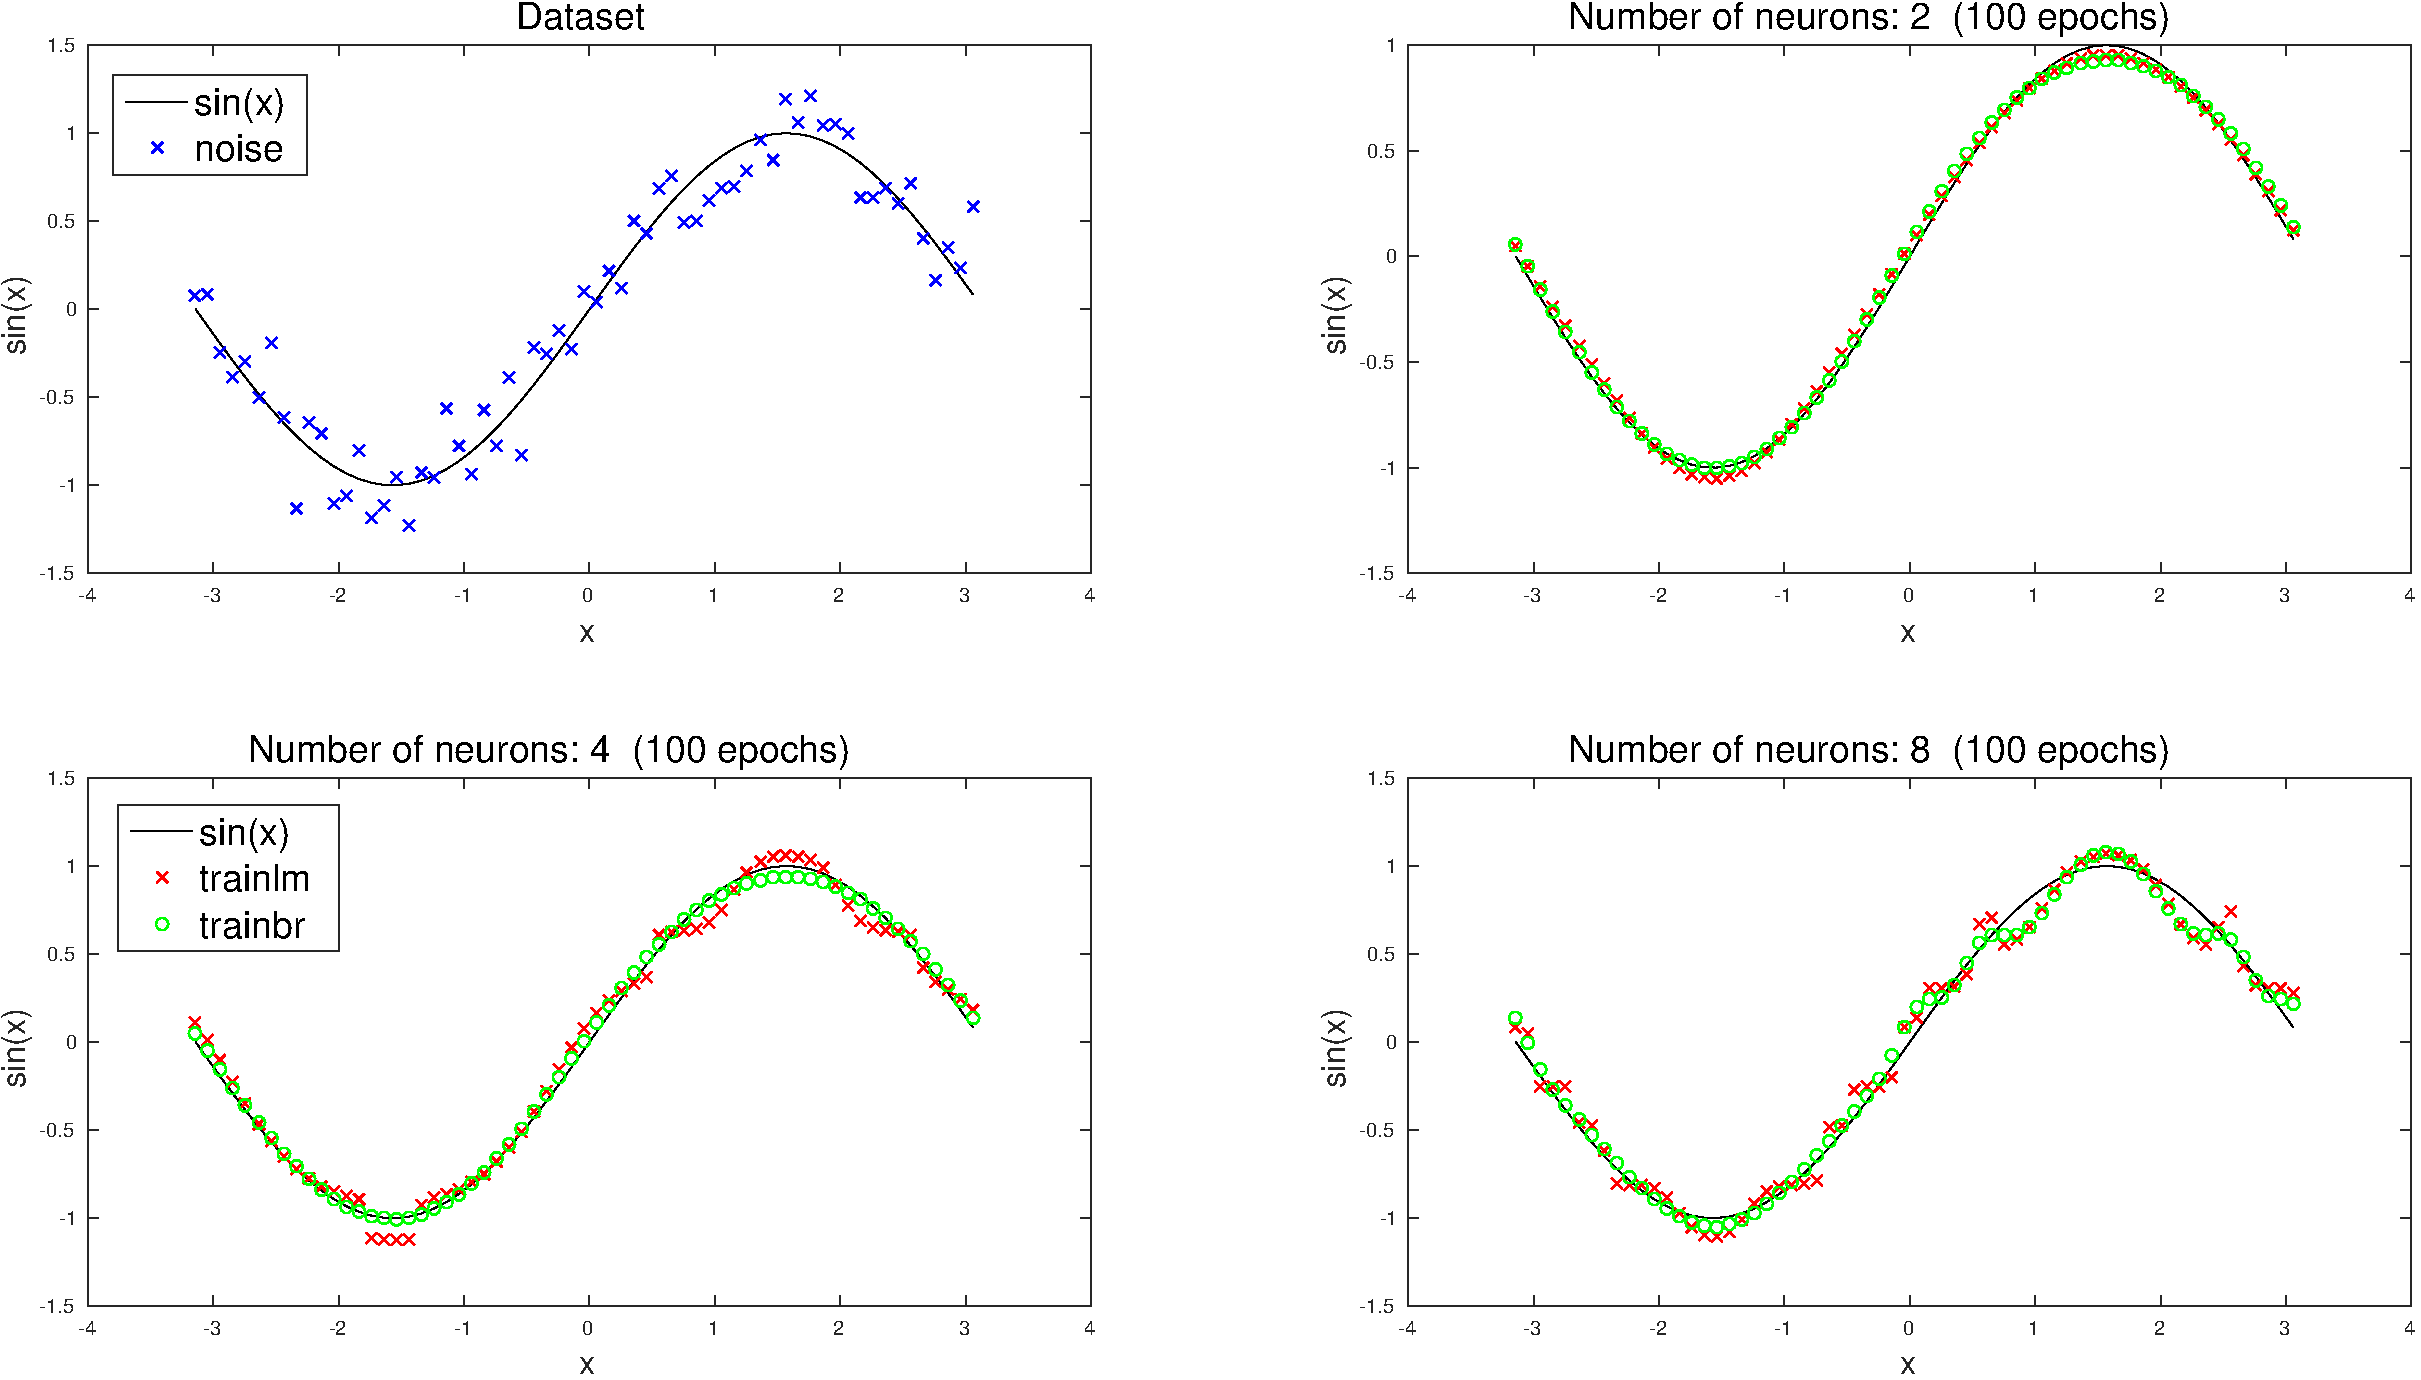
\includegraphics[scale=.40]{bayes_trainbrlm.pdf}
  \caption{Influence of number of neurons on the function estimation}
  \label{fig:trainbr}
\end{figure}

\begin{wrapfigure}{r}{0.7\textwidth}
  \vspace{-30pts}
  \begin{center}
    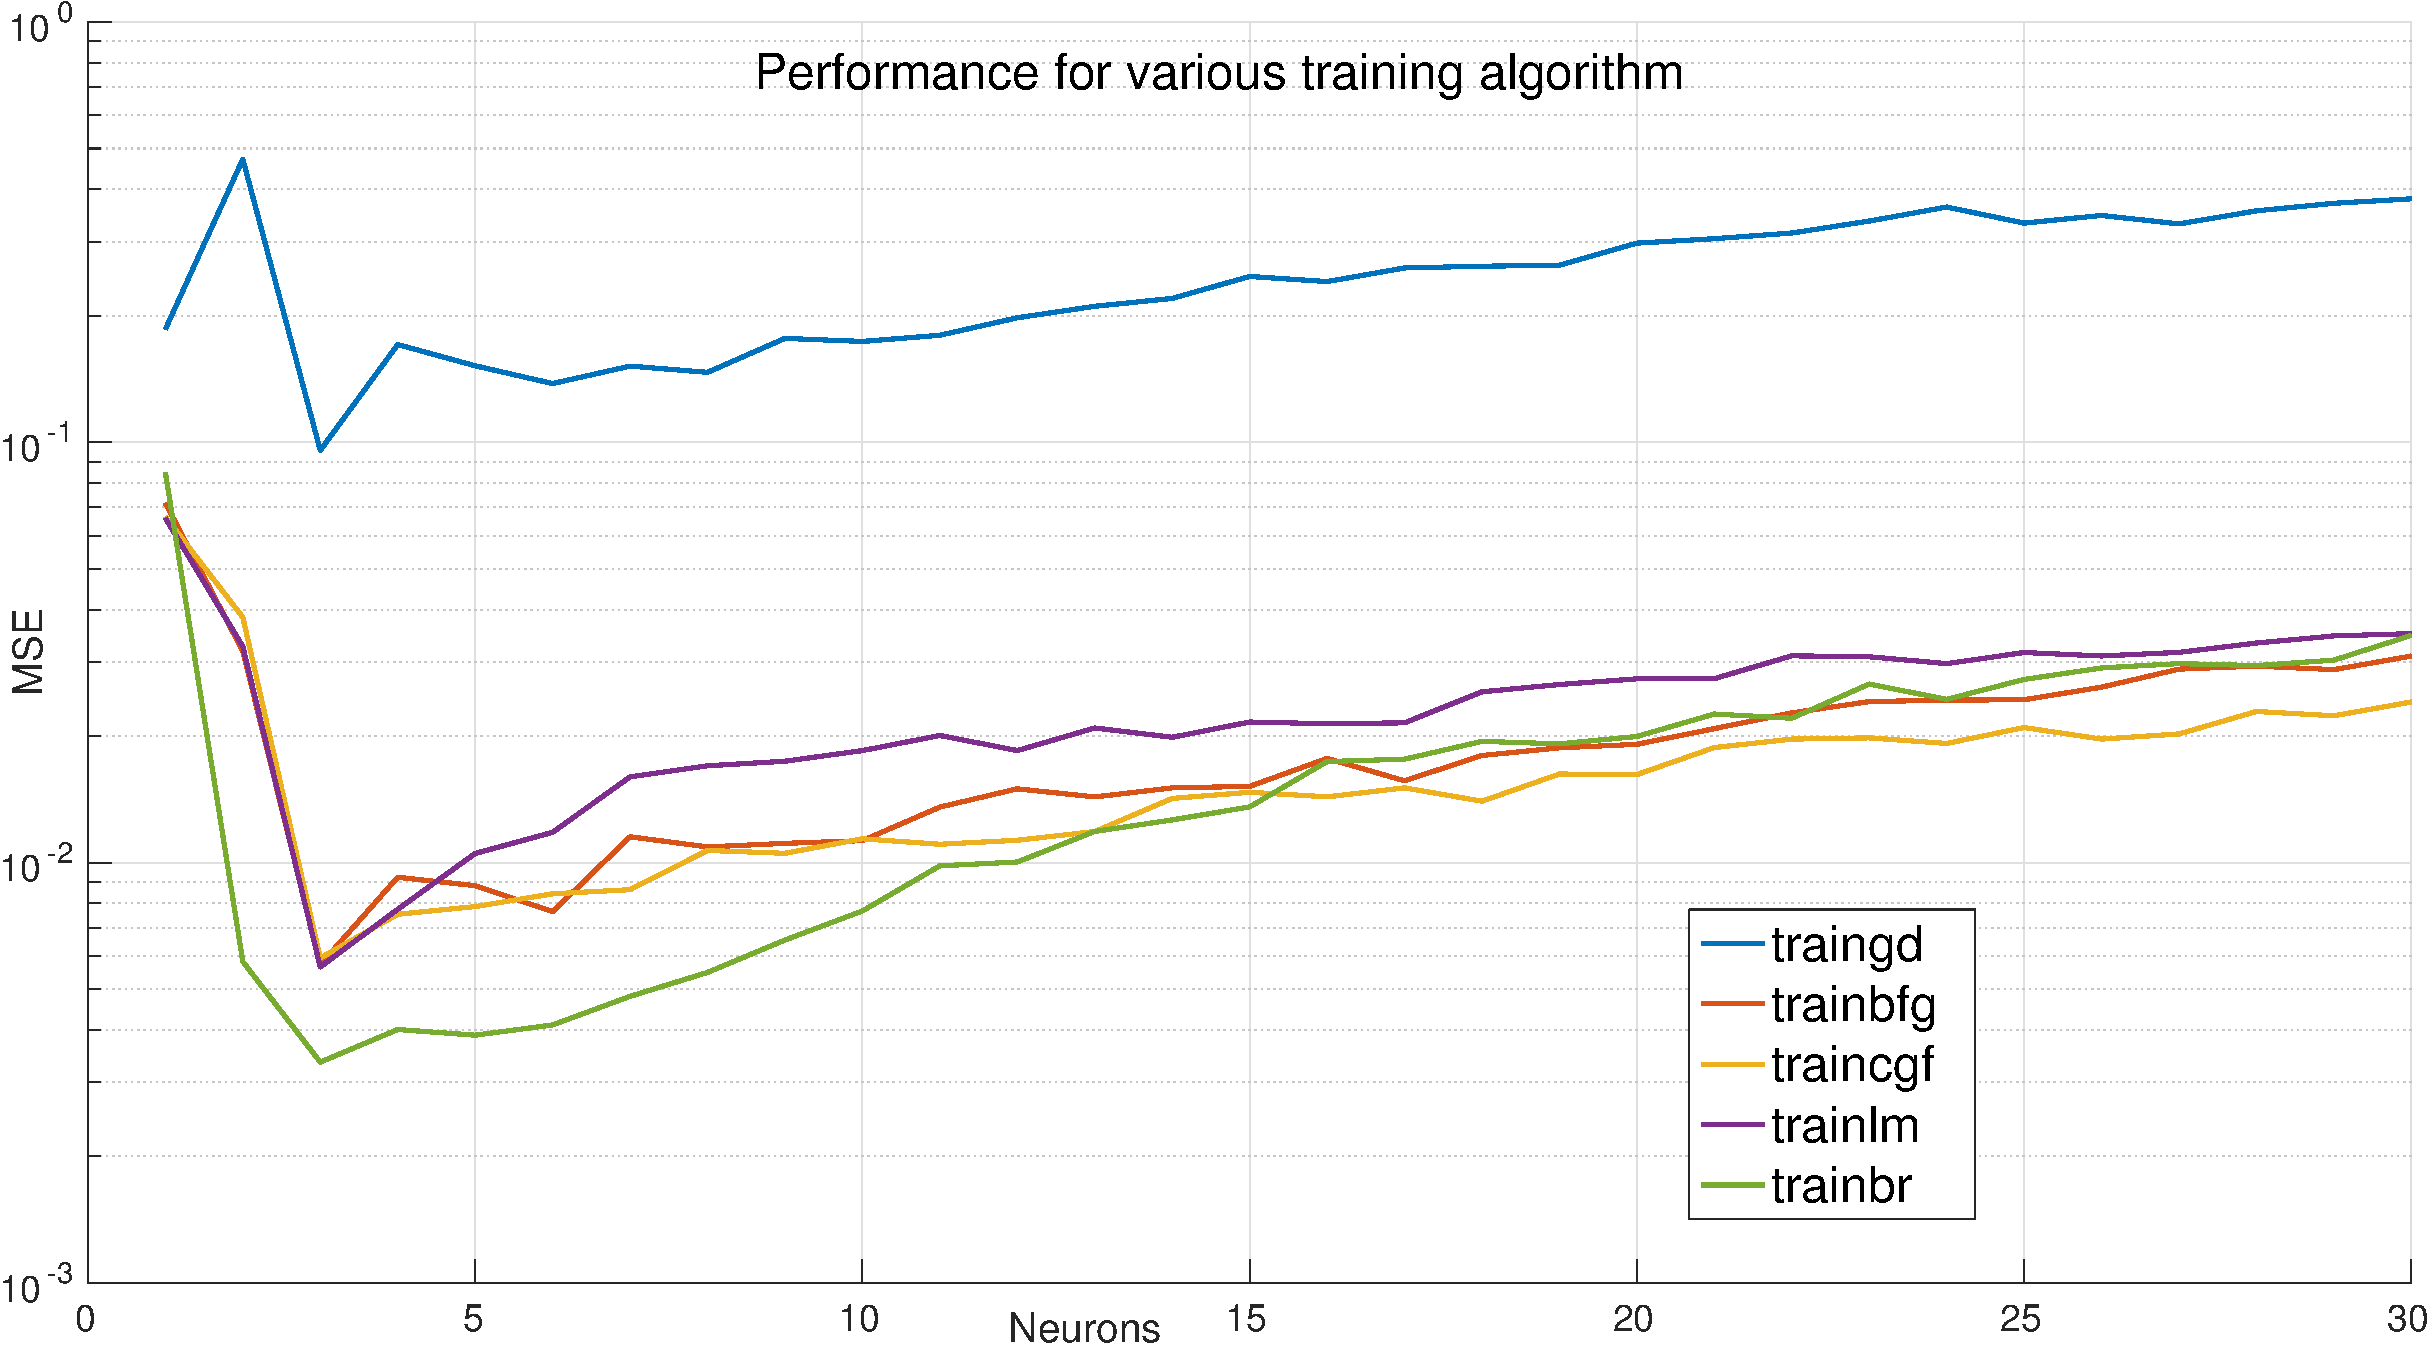
\includegraphics[width=0.7\textwidth]{true_mse_perf.pdf}
  \end{center}
\end{wrapfigure}

To investigate further, I took a look at the performance of the
networks using the performance function MSE for different models. This
is only possible because we know the true underlying
function. Otherwise, I would have used a resampling approach, such as
10-fold cross validation. The results are reported on the right, for
each architecture (parameter = number of neurons, and choice of
training algorithm), I fixed the number of epochs to 1000, then
proceeded to build 50 different datasets. For each, the performance
was evaluated, and then averaged over the 50 datasets.

As can be seen on the plot above and on the right, the \emph{trainbr}
performs indeed well in the region of few neurons compared to other
algorithms.

\end{document}
